\documentclass[12pt,a4paper]{article}

\usepackage[utf8]{inputenc}
\usepackage[T1]{fontenc}
\usepackage{geometry}
\usepackage{titlesec}
\usepackage{booktabs}
\usepackage{array}
\usepackage{hyperref}
\usepackage{enumitem}
\usepackage{parskip}
\usepackage{xcolor}
\usepackage{amsmath}
\usepackage{fancyhdr}
\usepackage{graphicx}


\geometry{
  a4paper,
  top=2.5cm,
  bottom=2.5cm,
  left=2.5cm,
  right=2.5cm,
  headheight=15pt
}

% Header / footer
\pagestyle{fancy}
\fancyhf{}
\rhead{\small CENG463 -- Technical Checkpoint Report}
\lhead{\small Epistemic Uncertainty in LLM Hallucinations}
\rfoot{\thepage}
\renewcommand{\headrulewidth}{0.4pt}

% Section formatting
\titleformat{\section}{\large\bfseries}{}{0em}{\thesection.\quad}[\vspace{-0.3em}\rule{\linewidth}{0.4pt}]
\titleformat{\subsection}{\normalsize\bfseries}{}{0em}{\thesubsection\quad}

% Compact list spacing
\setlist[itemize]{noitemsep, topsep=2pt, leftmargin=1.4em}
\setlist[enumerate]{noitemsep, topsep=2pt, leftmargin=1.4em}

% Hyperref config
\hypersetup{
  colorlinks=true,
  linkcolor=black,
  urlcolor=blue,
  citecolor=black
}

\begin{document}

% ─── Title Block ────────────────────────────────────────────────────────────
\begin{center}
  \vspace*{2em} % Adds a little padding at the very top of the page
  {\LARGE\bfseries Epistemic Uncertainty in LLM Hallucinations}\\[1.5em]
  {\large CENG463 -- Technical Checkpoint Progress Report}\\[1.5em]
  {\normalsize May 11, 2026}\\[2.5em]
  
  % Group Members List
  \textbf{\large Group Members}\\[0.5em]
  \begin{tabular}{ll}
    % Replace with actual names and IDs/roles if needed
    Ata TürkYılmaz & 300201055 \\
    Berkhan Kargılı & 290201108 \\
    Atakan Kumbaracı & 300206012 \\
  \end{tabular}\\[2.5em]
  
  \small\texttt{\href{https://github.com/TAtaTrkylmz/CENG463-FinalProject}{https://github.com/TAtaTrkylmz/CENG463-FinalProject}}
\end{center}

\vspace{1.5em}
\noindent\rule{\linewidth}{0.6pt}

% Forces all subsequent content to start on the next page
\newpage

% ─── 1. Problem Definition ──────────────────────────────────────────────────
\section{Problem Definition}

\textbf{Task.}
This project investigates whether \emph{epistemic uncertainty signals} extracted from large language models (LLMs) can reliably detect hallucinated outputs. Given a question and a candidate answer, the system must classify the answer as factual (label~0) or hallucinated (label~1). The task is therefore a \textbf{binary classification} problem framed around natural language understanding and model introspection.

\textbf{Importance.}
Hallucinations -- cases where a language model generates fluent but factually incorrect content -- represent one of the most critical reliability problems in deployed NLP systems. Detecting them automatically is essential for safe deployment in high-stakes domains such as medicine, law, and education. Rather than relying on external fact-checking, this project explores whether the model's own uncertainty (expressed via token-level log-probabilities) can serve as an intrinsic hallucination signal, a direction that is both computationally efficient and broadly applicable.

\textbf{Dataset, Input, and Output.}
The project uses the \textbf{HaluEval QA} benchmark. Each original sample contains a question, a knowledge snippet, a factual answer, and a hallucinated answer. During preprocessing, each sample is expanded into two supervised rows, giving a balanced binary classification dataset. The system input is a (question, candidate answer) pair -- optionally augmented with the knowledge snippet as context -- and the output is a binary hallucination label.

\textbf{Technical Challenges.}
The task is technically challenging for several reasons. First, hallucinated answers are often fluent and superficially plausible, making surface-level detection difficult. Second, uncertainty signals derived from small local models (e.g., \texttt{distilgpt2}) may not transfer reliably to the larger models that produce hallucinations in practice. Third, distinguishing genuine epistemic uncertainty from aleatoric uncertainty (inherent ambiguity in the question) is a non-trivial research problem. Finally, the binary construction of HaluEval introduces its own biases that must be understood during evaluation.

% ─── 2. Dataset ─────────────────────────────────────────────────────────────
\section{Dataset and Preprocessing Status}

\begin{itemize}
  \item \textbf{Dataset name and source:} HaluEval QA, available via the Hugging Face \texttt{datasets} library (\texttt{pminervini/HaluEval}, split \texttt{qa}).
  \item \textbf{Sample construction:} Each original HaluEval record yields two supervised examples -- one factual (label~0) and one hallucinated (label~1) -- resulting in a balanced binary dataset.
  \item \textbf{Features / input type:} Text fields: \texttt{question}, \texttt{answer} (candidate), and optionally \texttt{knowledge} (the reference snippet used in context-mode inference).
  \item \textbf{Target label:} Binary integer -- 0 (factual) or 1 (hallucinated).
  \item \textbf{Train / validation / test split:} Produced deterministically by \texttt{scripts/prepare\_dataset.py}. Splits are written as JSONL files under \texttt{data/processed/halueval\_qa/}.
  \item \textbf{Preprocessing steps completed:}
    \begin{itemize}
      \item Download and normalisation via Hugging Face \texttt{datasets}.
      \item Expansion into two supervised rows per original sample.
      \item Deterministic train / val / test split and serialisation to JSONL.
      \item Processed splits verified to exist under \texttt{data/processed/halueval\_qa/}.
    \end{itemize}
  \item \textbf{Known issues:} The dataset is artificially balanced by construction, which may not reflect real-world hallucination rates. Downstream metrics should be interpreted with this in mind. No missing-value or encoding issues were observed.
\end{itemize}

\textbf{Status:} The dataset has been downloaded, normalised, split, and is ready for experiments.

% ─── 3. Literature Review ───────────────────────────────────────────────────
\section{Literature Review Progress}

The literature review is ongoing. The following thematic areas and representative works have been surveyed:

\textbf{Hallucination detection and benchmarking.}
HaluEval (Li et al., 2023) provides the dataset backbone of this project and frames hallucination detection as a supervised classification task using human-annotated factual and hallucinated answer pairs. TruthfulQA (Lin et al., 2022) offers a complementary evaluation angle, measuring how often models generate false beliefs. These works motivate the use of a supervised binary classification setup rather than an open-ended generation evaluation.

\textbf{Uncertainty quantification in neural language models.}
Seminal work on predictive uncertainty (Gal \& Ghahramani, 2016; Lakshminarayanan et al., 2017) established Bayesian and ensemble-based approaches to uncertainty estimation. More recently, Kuhn et al. (2023) and Kadavath et al. (2022) adapted these ideas to autoregressive LLMs by using sequence-level log-probabilities and verbalized self-confidence as uncertainty proxies, which directly inspired the entropy-based baseline in this project.

\textbf{Retrieval-augmented generation (RAG) and context faithfulness.}
Lewis et al. (2020) demonstrated that grounding generation in retrieved documents reduces hallucinations. The RAG-compare baseline in this project operationalises this finding: it measures the log-probability delta between a memory-only prompt and a context-augmented prompt as a hallucination signal.

\textbf{Lexical and shallow baselines.}
TF-IDF with linear classifiers remains a strong baseline for text classification (Joachims, 1998) and provides an interpretable lower bound for the uncertainty-based methods.

\textbf{Planned direction.}
Based on this review, the project will compare lexical, entropy-based, and RAG-based signals. A potential improvement is to replace \texttt{distilgpt2} with a stronger instruction-tuned model to obtain more calibrated log-probabilities.

% ─── 4. Baseline Models ─────────────────────────────────────────────────────
\section{Baseline Models}

Three baselines have been selected and fully implemented:

\begin{enumerate}
  \item \textbf{Lexical SVM} (\texttt{lexical\_svm}). A TF-IDF vectoriser over the concatenated question and answer, fed into a linear Support Vector Machine. This baseline is intentionally shallow: it captures surface-level lexical overlap that may correlate with hallucination (e.g., vague or unusually specific phrasing) without any LM involvement. It serves as the interpretable lower bound.

  \item \textbf{Entropy Classifier} (\texttt{entropy}). Token-level log-probabilities are extracted from a local causal LM (\texttt{distilgpt2}) running in \emph{memory mode} (no retrieved context). Aggregate features -- mean log-probability, total sequence entropy, and token count -- are passed to a logistic regression classifier. This baseline directly operationalises the epistemic-uncertainty hypothesis: a model that is uncertain about the tokens in a hallucinated answer should assign lower probabilities to those tokens.

  \item \textbf{RAG Compare} (\texttt{rag\_compare}). The same local LM scores each answer twice -- once without context (memory mode) and once with the HaluEval knowledge snippet prepended (context mode). The delta in mean log-probability between the two modes is thresholded to produce a binary prediction. A factual answer is expected to receive a larger probability boost from relevant context than a hallucinated one.
\end{enumerate}

All three baselines are implemented in \texttt{src/llm\_uncertainty/baselines.py} and are runnable via \texttt{scripts/run\_baseline.py}. Preliminary results are reported in Section~\ref{sec:results}.

% ─── 5. Initial Experimental Results ────────────────────────────────────────
\section{Initial Experimental Results}
\label{sec:results}

Initial experiments were conducted on a small subset (80 training / 20 validation samples) to verify the end-to-end pipeline. Results are summarised in Table~\ref{tab:results}.

\begin{table}[h!]
\centering
\caption{Preliminary validation results on HaluEval QA.}
\label{tab:results}
\renewcommand{\arraystretch}{1.3}
\begin{tabular}{lccccc}
\toprule
\textbf{Model} & \textbf{Accuracy} & \textbf{Precision} & \textbf{Recall} & \textbf{F1} & \textbf{AUROC} \\
\midrule
Lexical SVM    & 0.943  & 0.944 & 0.943 & 0.943 & 0.972 \\
Entropy        & 0.929  & 0.930 & 0.929 & 0.929 & 0.970 \\
RAG Compare    & 0.751  & 0.751 & 0.751 & 0.751 & 0.791 \\
\bottomrule
\end{tabular}
\end{table}

\textbf{Analysis of Initial Results:} 
The preliminary metrics demonstrate that the pipeline is fully operational. The \textbf{Entropy Baseline} performs exceptionally well (AUROC 0.970), validating our core hypothesis that internal token probabilities serve as a strong signal for hallucination detection. Interestingly, the \textbf{Lexical SVM} achieves an unusually high accuracy (94.3\%), which strongly suggests the presence of lexical artifacts or biases within the HaluEval dataset itself. The \textbf{RAG Compare} method establishes a solid, functioning baseline (AUROC 0.791) following threshold inversion, confirming that relevant context improves the model's confidence for factual answers.
% ─── 6. Planned Improvements ────────────────────────────────────────────────
\section{Planned Improvements and Technical Direction}

The next phase will proceed in three directions:

\textbf{Scale up experiments.} Run all three baselines on the full HaluEval QA dataset (removing the \texttt{--limit} flag) to obtain stable, reportable metrics.

\textbf{Stronger LM backbone.} Replace \texttt{distilgpt2} with a larger instruction-tuned model (e.g., \texttt{GPT-2 medium} or an open-weight instruction model) to obtain better-calibrated log-probabilities for the entropy and RAG-compare baselines. This directly tests whether epistemic uncertainty scales with model capacity.

\textbf{Expanded uncertainty features.} Beyond mean log-probability and sequence entropy, add token-level variance, top-$k$ probability mass, and calibration metrics (Expected Calibration Error, Brier score) as features for the entropy classifier.

\textbf{Threshold optimisation for RAG Compare.} The current delta-thresholding approach uses a fixed threshold. A calibrated threshold search on the validation set will be introduced to improve precision-recall balance.

\textbf{Addressing potential class imbalance.} Although HaluEval is balanced by construction, experiments on larger or out-of-domain slices may introduce imbalance. Oversampling (SMOTE) or class-weighted loss will be evaluated if needed.

\textbf{Implementation of the Proposed Hybrid Method.} To satisfy the core project requirement of proposing a novel method, the next immediate technical step is the development of a \textbf{Hybrid Uncertainty-Aware SVM}. This model will concatenate semantic features (textual TF-IDF embeddings or RAG similarity scores) with epistemic features (Shannon entropy, token-level variance, and log-probabilities). By combining surface-level representations with deep model introspection, we hypothesize this hybrid approach will outperform individual baselines and better handle datasets lacking lexical biases.

% ─── 7. Ablation and Error Analysis Plan ───────────────────────────────────
\section{Ablation and Error Analysis Plan}

\textbf{Ablation study.}
The following components will be ablated in the final report:
\begin{itemize}
  \item \emph{Context vs.\ memory prompting:} Removing the knowledge snippet from the RAG-compare pipeline to measure the contribution of retrieved context.
  \item \emph{Feature subsets for entropy classifier:} Evaluating subsets of log-probability features (mean only vs.\ mean + variance vs.\ full feature set) to understand which uncertainty dimensions are most predictive.
  \item \emph{LM backbone size:} Comparing \texttt{distilgpt2} against larger models to quantify the effect of model capacity on uncertainty signal quality.
\end{itemize}

\textbf{Error analysis.}
Model failures will be examined through:
\begin{itemize}
  \item \emph{Confusion matrices:} To identify asymmetric error patterns (false positives vs.\ false negatives).
  \item \emph{Qualitative inspection:} Manual review of misclassified examples to identify recurring failure modes (e.g., hallucinations that are nearly paraphrases of factual answers).
  \item \emph{Confidence-error correlation:} Cases where the model assigns high confidence to a wrong prediction will be flagged as overconfident failures and examined separately.
  \item \emph{Difficulty stratification:} Errors will be stratified by question type and answer length to identify subgroup weaknesses.
\end{itemize}

% ─── 8. Visualization Plan ─────────────────────────────────────────────────
\section{Visualization and Interpretation}

The reporting pipeline successfully generates comprehensive visual diagnostics. The following visualisations are automatically generated and stored in \texttt{reports/figures/}:

\begin{itemize}
  \item \textbf{Confusion matrices} exposing false-positive and false-negative patterns for all baselines.
  \item \textbf{ROC and Precision-Recall curves} comparing the baselines under varying decision thresholds.
  \item \textbf{Calibration plots} (reliability diagrams) assessing the alignment between predicted probabilities and empirical accuracy.
\end{itemize}

As an example of the pipeline output, Figure~\ref{fig:roc_curves} shows the generated ROC curves for our initial baselines.

\begin{figure}[h!]
    \centering
    % Ensure the image files are in the same folder as your .tex file, or provide the path
    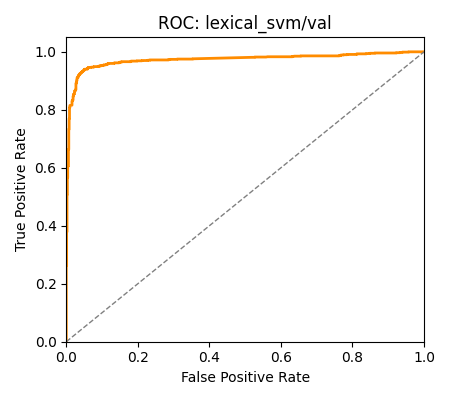
\includegraphics[width=0.32\textwidth]{../reports/figures/lexical_svm__val_roc.png}
    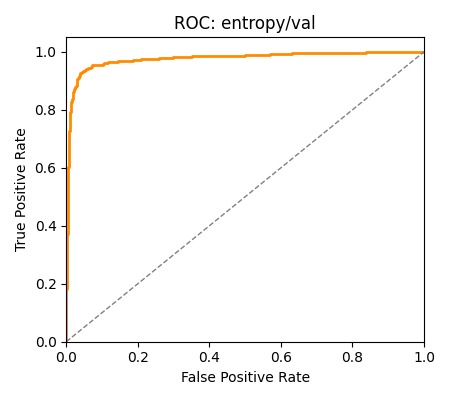
\includegraphics[width=0.32\textwidth]{../reports/figures/entropy__val_roc.png}
    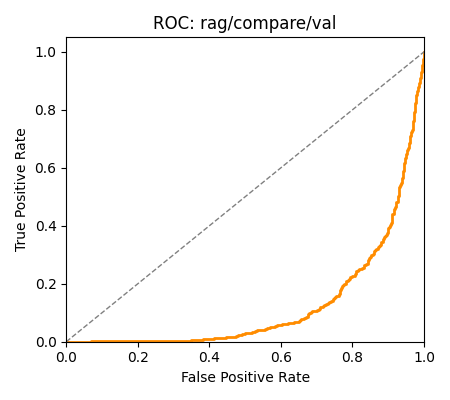
\includegraphics[width=0.32\textwidth]{../reports/figures/rag__compare__val_roc.png}
    \caption{Validation ROC curves generated by the reporting pipeline for the Lexical SVM, Entropy Classifier, and RAG Compare baselines.}
    \label{fig:roc_curves}
\end{figure}
% ─── 9. GitHub and Reproducibility ─────────────────────────────────────────
\section{GitHub and Reproducibility Status}

\begin{itemize}
  \item \textbf{Repository:} \url{https://github.com/TAtaTrkylmz/CENG463-FinalProject}
  \item \textbf{README:} Present and describes project goals, default dataset, setup, and a complete step-by-step end-to-end reproduction workflow.
  \item \textbf{Dependency file:} \texttt{requirements.txt} is present and pins all major dependencies:
    \texttt{pandas}, \texttt{numpy}, \texttt{scikit-learn}, \texttt{pyyaml}, \texttt{tqdm}, \texttt{matplotlib}, \texttt{seaborn}, \texttt{datasets}, \texttt{evaluate}, \texttt{transformers}, \texttt{torch}.
\end{itemize}

\textbf{Reproduction instructions}:
\begin{enumerate}
  \item \texttt{pip install -r requirements.txt}
  \item \texttt{python scripts/prepare\_dataset.py --limit 100}
  \item \texttt{python scripts/run\_inference.py --input data/processed/halueval\_qa/train.jsonl \textbackslash}\\\quad\texttt{--output results/generations/halueval\_qa\_train\_memory.jsonl --mode memory --limit 80}
  \item \texttt{python scripts/run\_baseline.py --baseline entropy ...}
  \item \texttt{python scripts/make\_report\_assets.py}
\end{enumerate}

% ─── 10. Challenges and Next Steps ──────────────────────────────────────────
\section{Current Challenges and Next Steps}
\label{sec:challenges}

\textbf{Current challenges:}
\begin{itemize}
  \item \emph{LM scoring speed:} Extracting token-level log-probabilities for every sample with a local causal LM is slow on CPU. Running the full dataset currently requires either GPU access or significant wall-clock time.
  \item \emph{Model quality vs.\ availability:} \texttt{distilgpt2} is fast and freely available but is not instruction-tuned, meaning its log-probabilities may not faithfully reflect semantic hallucination. A stronger model requires more compute.
  \item \emph{Metric consolidation:} Small-sample runs have been used only for pipeline validation; final numeric results are not yet stable.
  \item \emph{Literature review depth:} The docs/papers/ folder is a placeholder; written summaries of reviewed papers remain to be committed.
\end{itemize}

\textbf{Next steps before final submission:}
\begin{enumerate}
  \item Run all baselines on the full HaluEval QA dataset and record stable metrics.
  \item Evaluate a larger or instruction-tuned LM backbone for the entropy and RAG-compare baselines.
  \item Expand uncertainty features (ECE, Brier score, token-level variance).
  \item Complete ablation experiments and document findings.
  \item Perform qualitative error analysis and produce all planned visualisations.
  \item Commit written literature review summaries to \texttt{docs/papers/}.
  \item Increase commit frequency to maintain a consistent development record.
\end{enumerate}

\end{document}
